\documentclass{article}
\usepackage{graphicx}
\usepackage[margin=1.5cm]{geometry}
\usepackage{amsmath}
\usepackage{hyperref}

\begin{document}

\title{Week 6 Writing Activity: Technical Description I}
\author{Prof. Jordan C. Hanson (INTD100)}

\maketitle

\section{Technical Description I}

\textit{Many people think they can describe something.} - Have you ever been in a situation in which you were \textit{sure} someone understood you, only to find out they had the wrong idea?  What is required of good technical description?
\begin{figure}[ht]
\centering
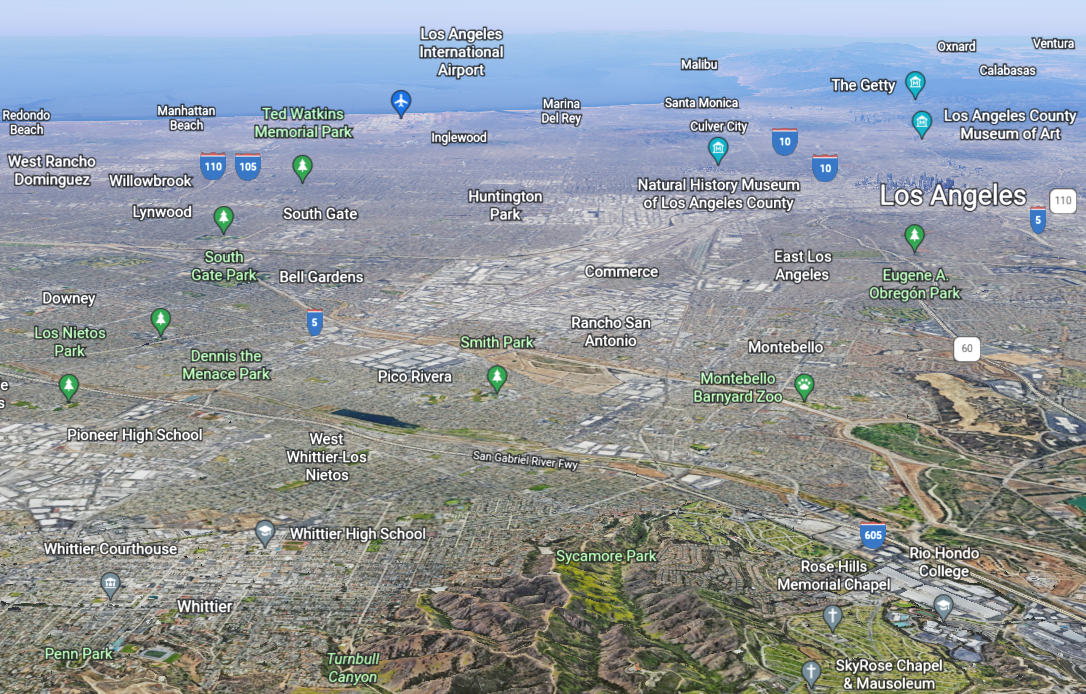
\includegraphics[width=0.5\textwidth]{map.png}
\caption{\label{fig:1} A map of our local area within Southern California.}
\end{figure}

\begin{enumerate}
\item (a) Which cardinal direction corresponds to \textit{upwards} in the map shown in Fig. \ref{fig:1}?  Note the location of the ocean, Los Angeles International Airport, and Whittier. (b) Write an unambiguous set of directions that takes the reader from where you live to this classroom.  Your writing should be \textit{repeatable} by someone unfamiliar with your route. \\ \vspace{1cm}
\item In \textit{The Scientific Attitude}, Chapter 5, the author identifies (6) ways in which scientists intent on proving something regardless of whether it is warranted or not:
\begin{enumerate}
\small
\item Cherry picking data (taking only the \textit{good} data).
\item Curve fitting (manipulating data until it matches a theoretical curve).
\item Continuing to take data until the desired results are found.
\item Excluding data (excluding the \textit{bad} data).
\item Using a small data set.
\item P-hacking (\url{https://xkcd.com/882/}).
\end{enumerate}
Choose three of these tactics, and explain below how writing \textit{unambiguously} protects everyone from these forms of scientific fraud.
\end{enumerate}

\end{document}
